\section{Time Performance}\label{section:timePerformance}

Another important property is the time of the local view template building and especially the time of comparing two templates. The time of the template building and comparing the two templates are measured separately. The reason is that the template building is done only once per scene, independently of the length of the algorithm's run. However, comparing the two templates is done more times for every scene. Namely, every new scene is compared with all previously saved scenes whose number increases over time, especially in large and various environments. Therefore, the time of the matching is the critical part and must be as fast as possible. In contrast, the time of the building can be significantly larger as long as it stays smaller than the period between two sensor inputs.\par
The system was tested on a Laptop with the following parameters:

\begin{description}[labelwidth=5em,leftmargin =\dimexpr\labelwidth+\labelsep\relax]
    \item[\textbf{Processor}:] Intel${}^{\text{\tiny{\textregistered}}}$ Core™ i7-8650U Processor (1.9 - 4.2 GHz) \footnote{\tiny{\url{https://ark.intel.com/content/www/us/en/ark/products/124968/intel-core-i7-8650u-processor-8m-cache-up-to-4-20-ghz.html}}}
    \item[\textbf{RAM}:]
          \begin{itemize}
              \item 4 GiB Row of chips DDR4 Synchronous Unbuffered (Unregistered) 2400 MHz (0,4 ns)
              \item 8 GiB SODIMM DDR4 Synchronous Unbuffered (Unregistered) 2400 MHz (0,4 ns)
          \end{itemize}
    \item[\textbf{OS}:] Kubuntu 21.10 x86\_64,
\end{description}

inside of the virtual machine, with the following limitations and operating system:

\begin{description}[labelwidth=5em]
    \item[\textbf{RAM}:] 8 GiB
    \item[\textbf{OS}:] Ubuntu 20.04 LTS x86\_64.
\end{description}

The GPU did not have CUDA support, so all the computations were performed on a CPU.\par
The figures \ref{fig:timesWarehouse}, \ref{fig:timesHouse}, and \ref{fig:timesHospital} show the LV building times for each scene and also matching times for each pair of compared scenes in all the environments. The table \ref{tab:averageTimes} shows the average times for each approach in every environment compared with the visual place recognition used in the original RatSLAM.


\begin{figure}[!tbp]
    \centering
    \subfloat[LV building times]{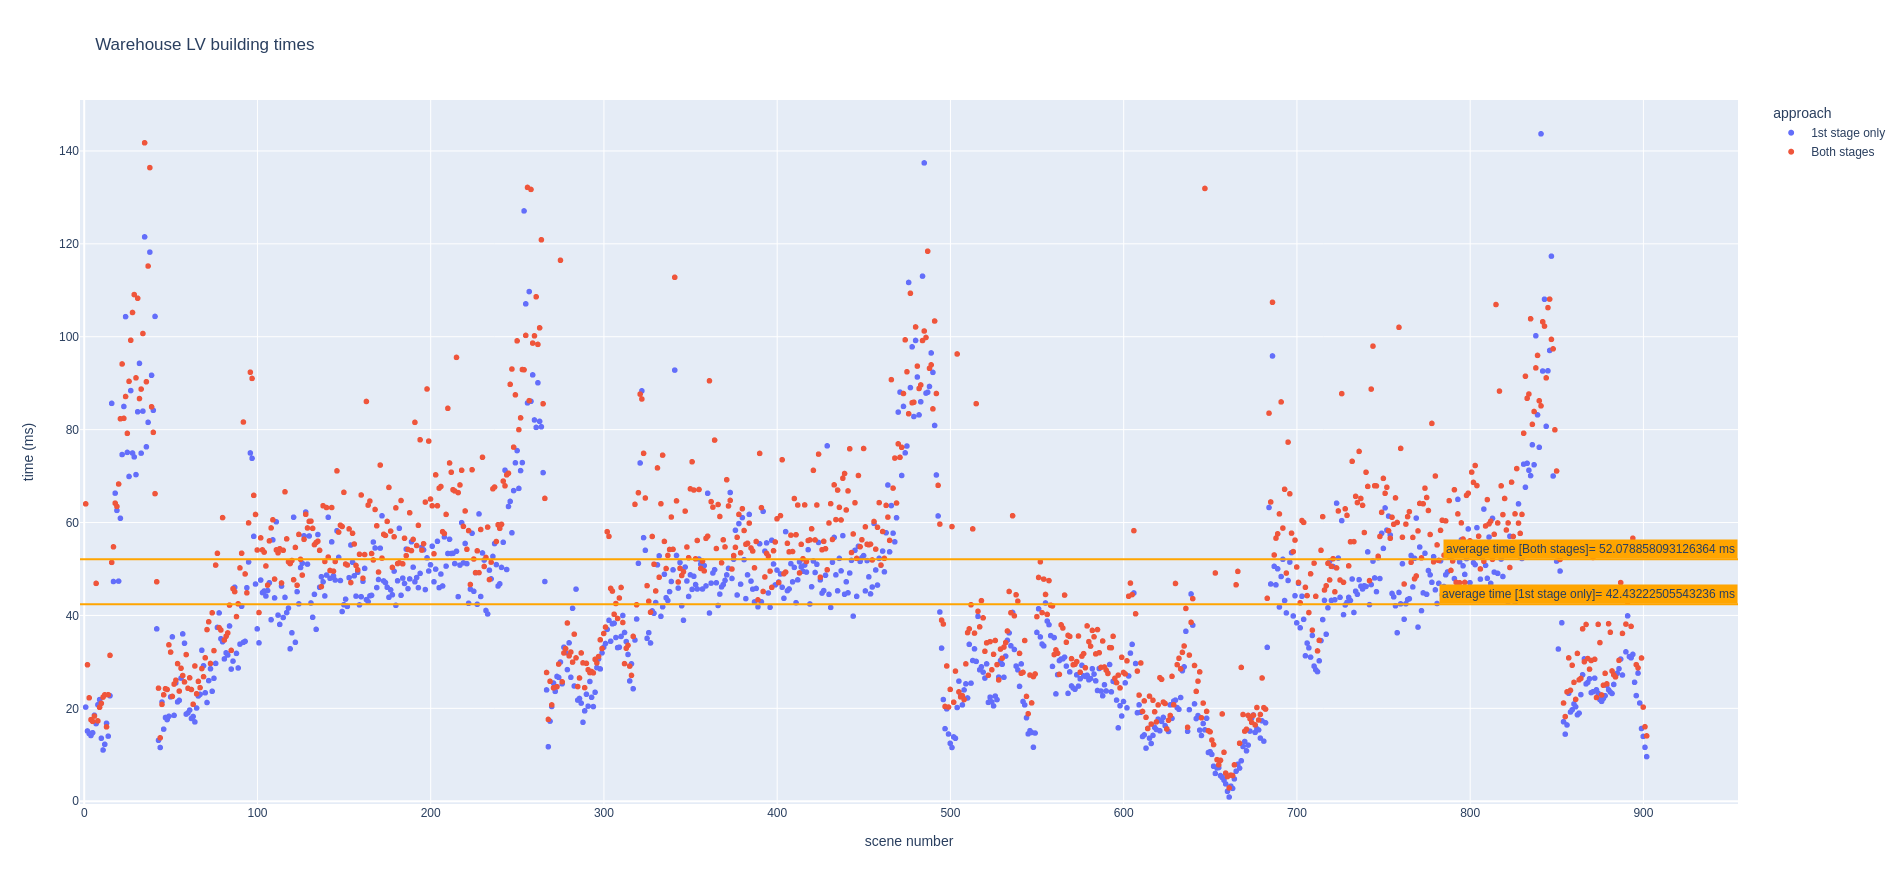
\includegraphics[width=0.8\textwidth]{warehouseBuildingTimes.png}\label{fig:timesWH1}}
    \\
    \subfloat[LV matching times]{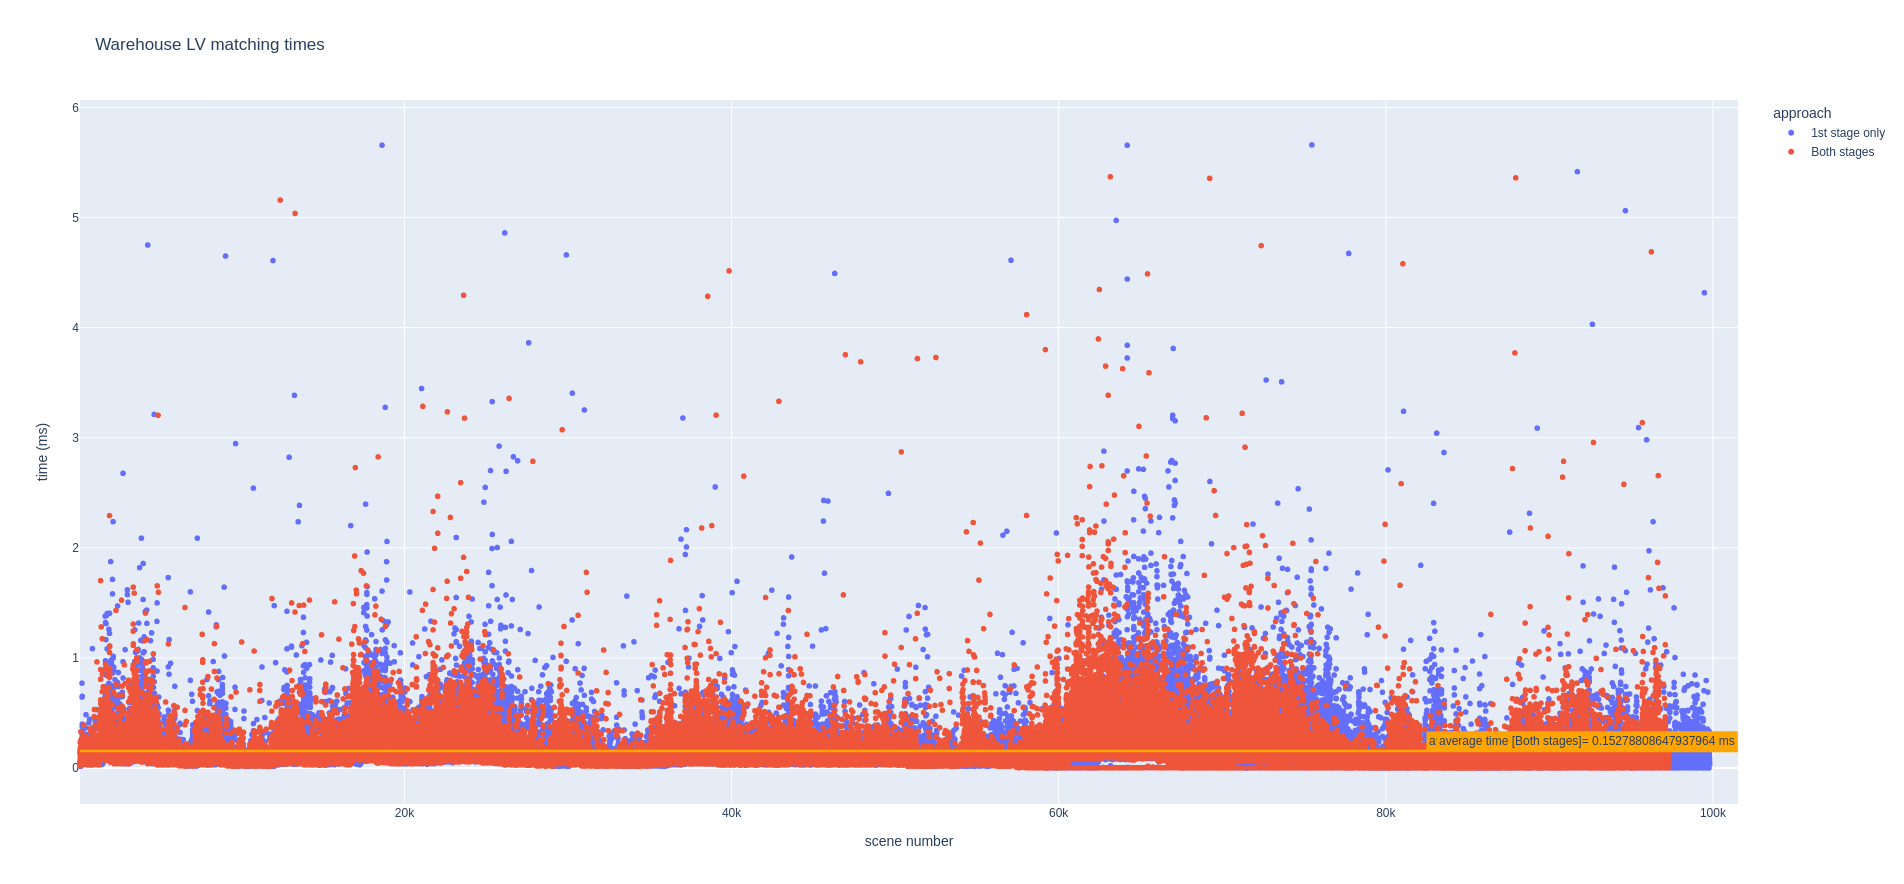
\includegraphics[width=0.8\textwidth]{warehouseMatchingTimes.png}\label{fig:timesWH2}}
    \caption{Computation times in the warehouse environment}
    \label{fig:timesWarehouse}
\end{figure}

\begin{figure}[!tbp]
    \centering
    \subfloat[LV building times]{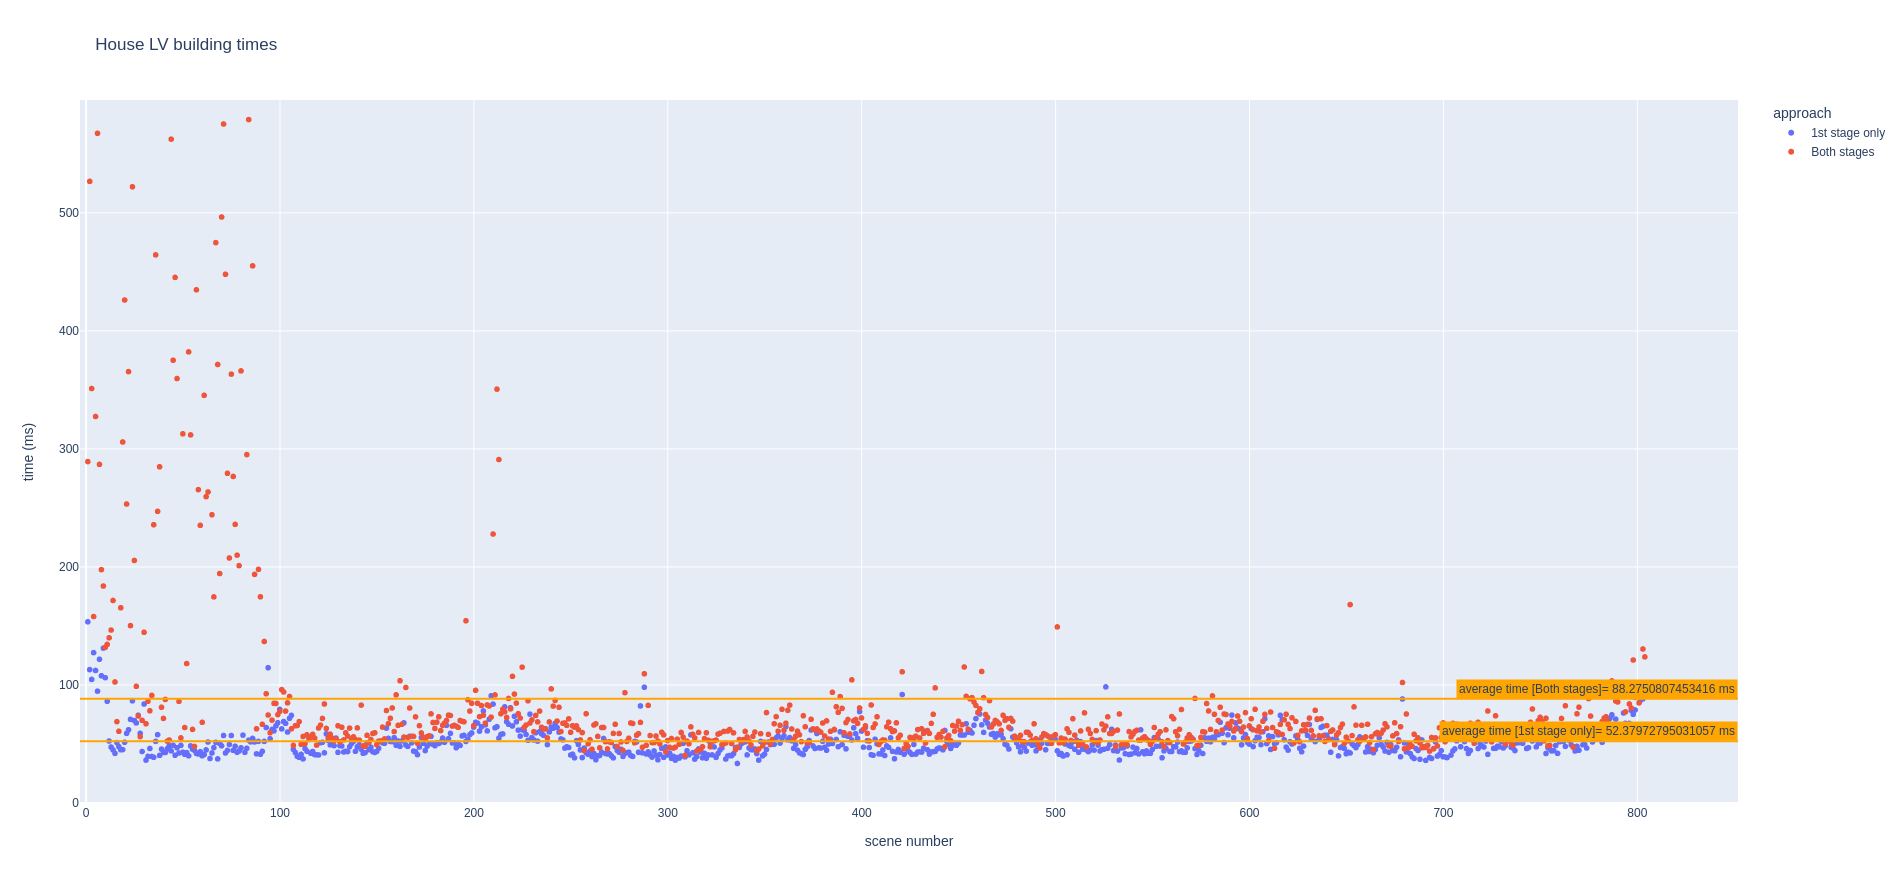
\includegraphics[width=0.8\textwidth]{houseBuildingTimes.png}\label{fig:timesHS1}}
    \\
    \subfloat[LV matching times]{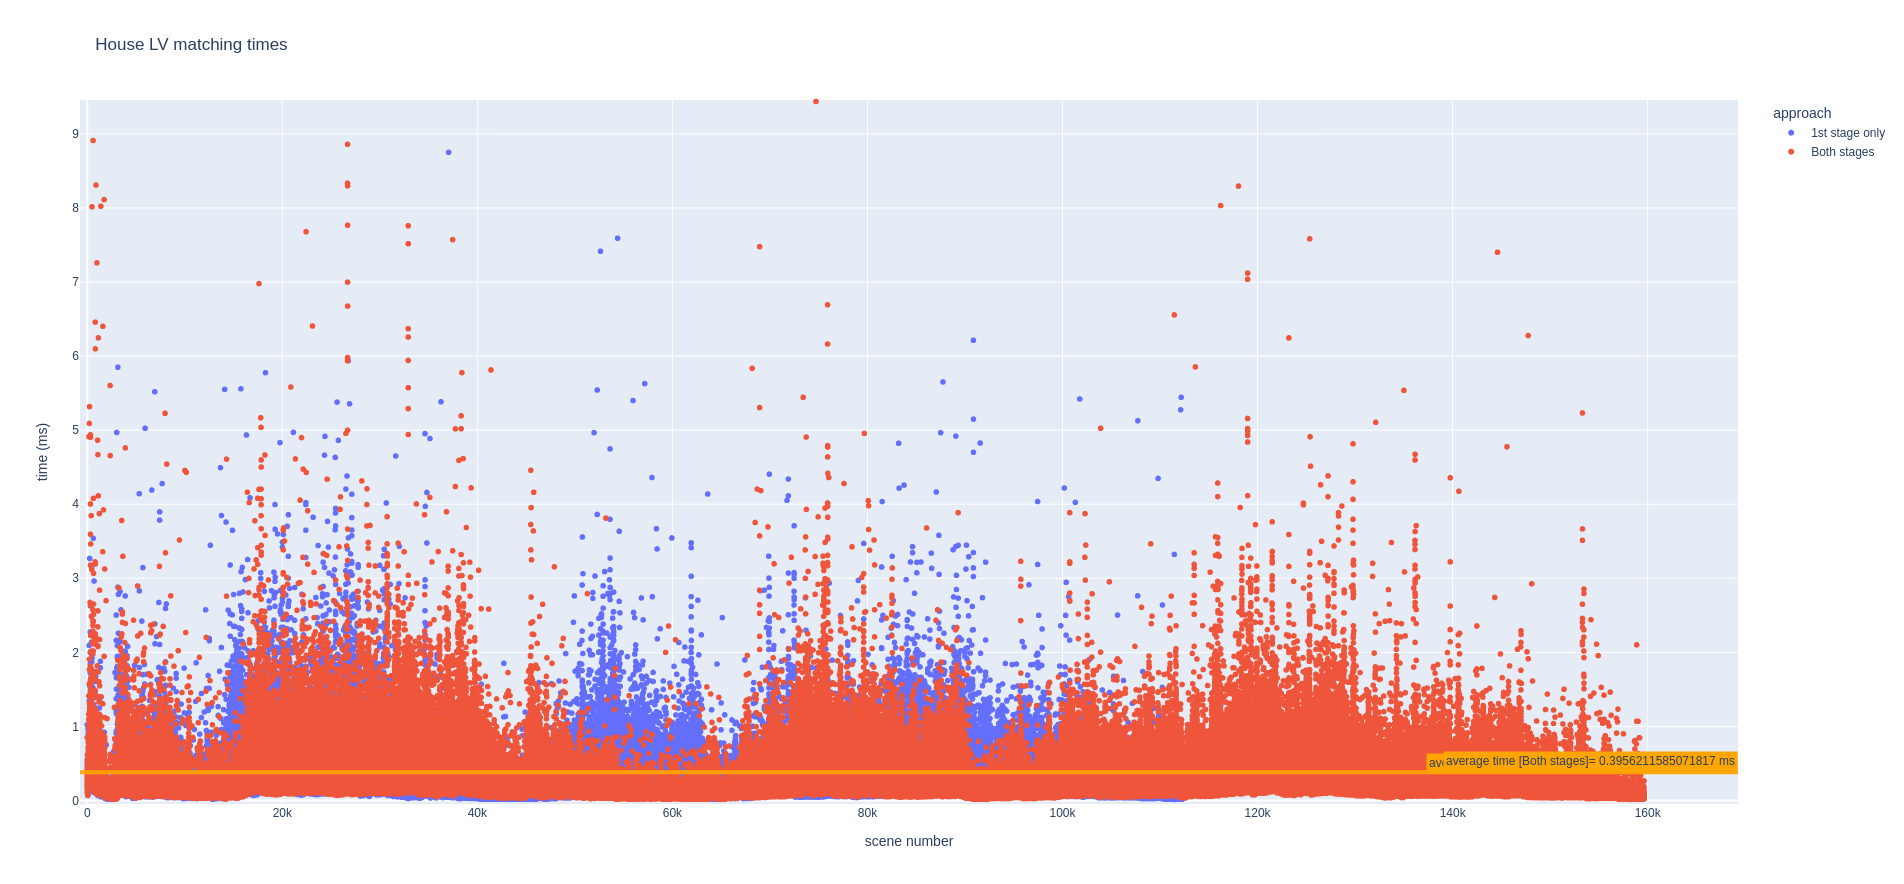
\includegraphics[width=0.8\textwidth]{houseMatchingTimes.png}\label{fig:timesHS2}}
    \caption{Computation times in the house environment}
    \label{fig:timesHouse}
\end{figure}

\begin{figure}[!tbp]
    \centering
    \subfloat[LV building times]{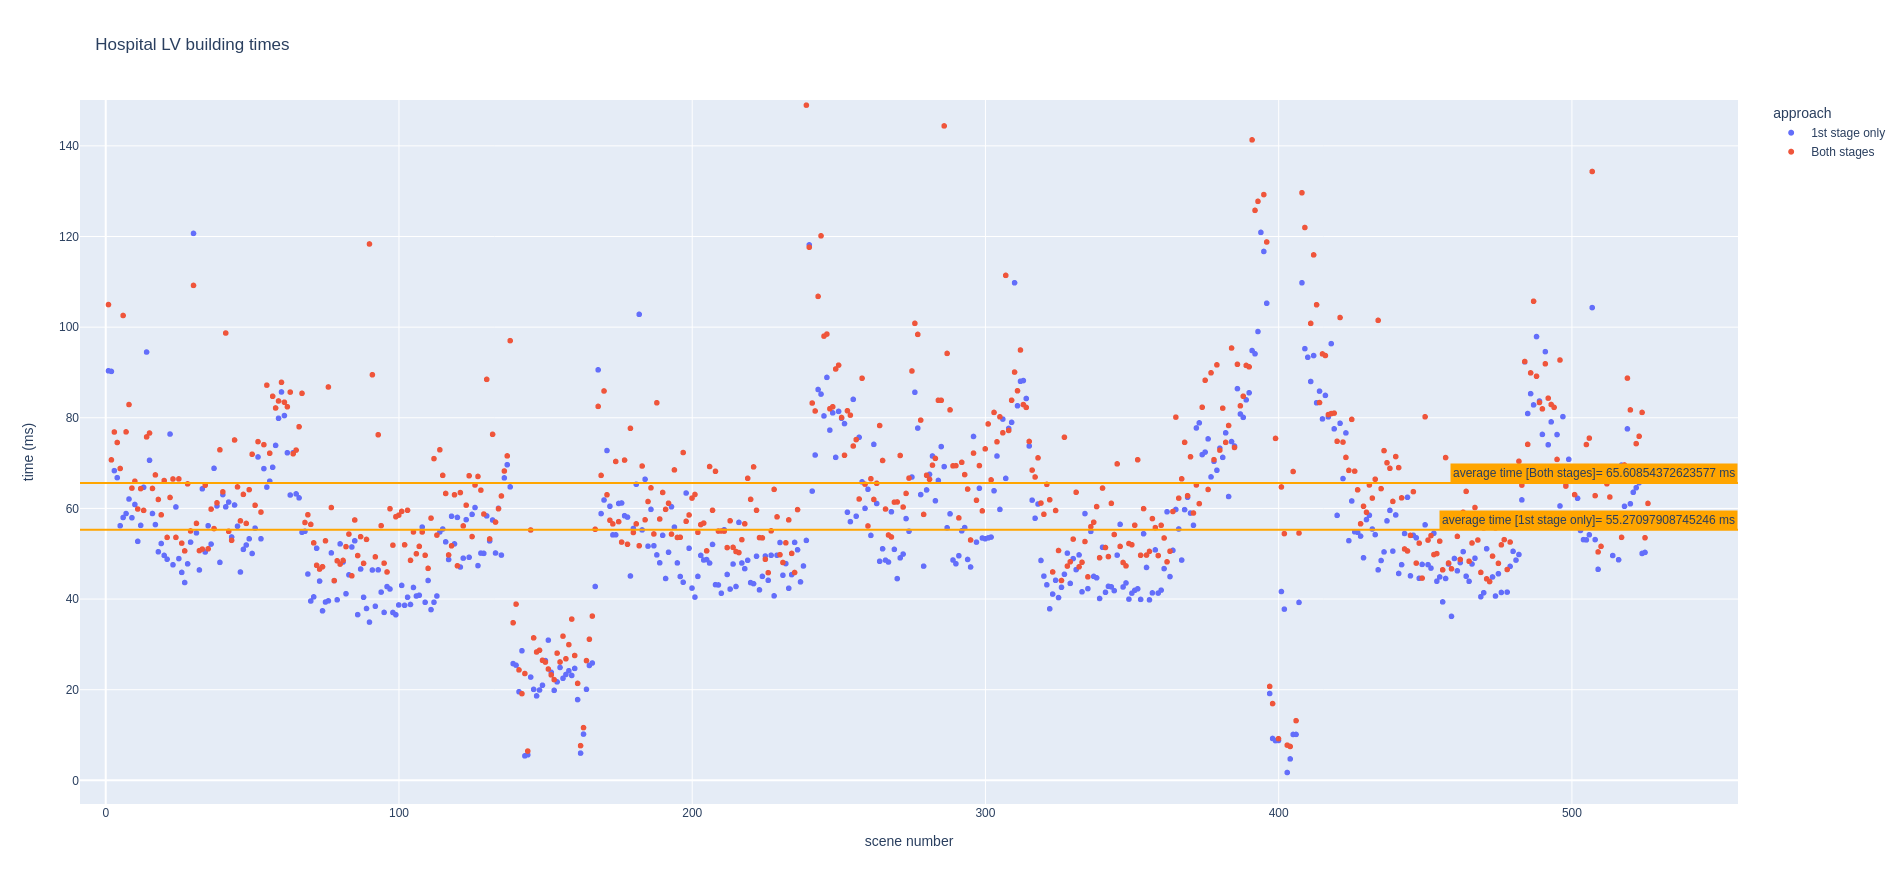
\includegraphics[width=0.8\textwidth]{hospitalBuildingTimes.png}\label{fig:timesHO1}}
    \\
    \subfloat[LV matching times]{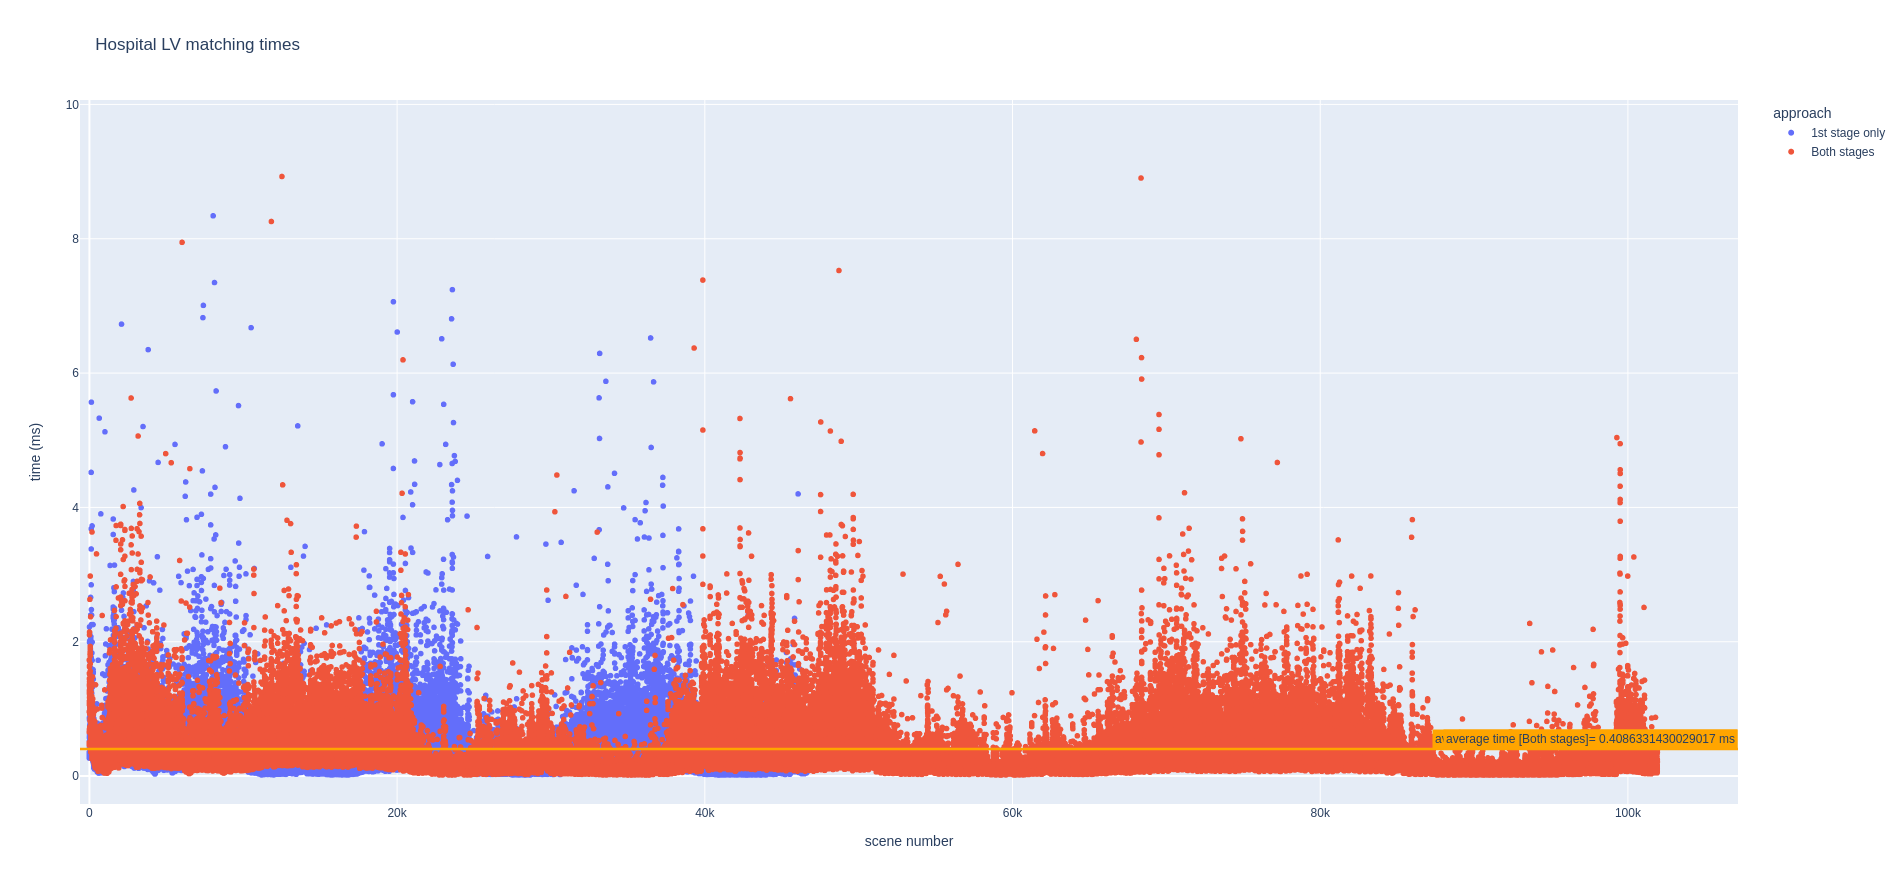
\includegraphics[width=0.8\textwidth]{hospitalMatchingTimes.png}\label{fig:timesHO2}}
    \caption{Computation times in the hospital environment}
    \label{fig:timesHospital}
\end{figure}

\begin{table}[htpb]
    \caption{Average times of LV matching and building in the different environments}\label{tab:averageTimes}
    \centering
    \begin{tabular}{l | l  l| l l| l l}
        \toprule
        \textbf{}               & \multicolumn{2}{l|}{\textbf{1st stage only}} & \multicolumn{2}{l|}{\textbf{both stages}} & \multicolumn{2}{l}{\textbf{original RatSLAM}}                                  \\
        {}                      & build                                        & match                                     & build                                         & match    & build    & match    \\
        \hline
        \textbf{Warehouse env.} & 42.432 ms                                    & 0.153 ms                                  & 52.078 ms                                     & 0.159 ms & 2.053 ms & 0.083 ms \\
        \textbf{House env.}     & 52.380 ms                                    & 0.396 ms                                  & 88.265 ms                                     & 0.368 ms & 1.448 ms & 0.137 ms \\
        \textbf{Hospital env.}  & 55.271 ms                                    & 0.399 ms                                  & 65.609 ms                                     & 0.409 ms & 1.762 ms & 0.092 ms \\
        \bottomrule
    \end{tabular}
\end{table}

The table and graphs show that the approach that uses only the first stage can build the local views considerably faster than the 2-stage approach. The time difference is caused by the feature extraction, which is present only in the 2-stage approach. However, the time difference is not so significant. Most importantly, the techniques are significantly faster than the frequency of the sensors, so the time performance of local view building of both methods is satisfactory. As we can see, the LV building is significantly slower than the LV building in the original RatSLAM. However, the original RatSLAM works with sensors with significantly higher frequency\footnote{In the experiments, the frequency of the camera was 15 times higher than frequency of the LiDAR.}, so the LV building is done significantly more often, and the total resources consumption of the LV building process is comparable with the total consumption of the approaches presented in this work.\par
The times of the view matching of both approaches are almost the same, so the overhead caused by feature comparison in the second stage is practically negligible. Even if the times are circa 2 to 4 times larger than the times measured by the original RatSLAM, the number of saved views is significantly smaller, as shown in table \ref{tab:memory}, so the total comparison time for each scene will be at the end smaller than in the original RatSLAM approach. Furthermore, the times are significantly smaller than 1 ms, so there could be saved up to a thousand different local views to compare until the total comparison time reaches the sensors period. This means that this approach will also be suitable for very long time runs in huge environments.
